\chapter{Pruebas y an'alisis de resultados}
\section{Prueba de adquisici'on de datos con el sensor HEDM-5500}
De esta prueba se obtuvo la siguiente gr'afica con una variaci'on de 2000 puntos de resoluci'on del sensor y 1500 muestras, como se muestra en la Fig.\ref{fig:adqsens}:
\setlength{\parskip}{0cm}
\begin{center}
\begin{figure}[ht]
	\centering
		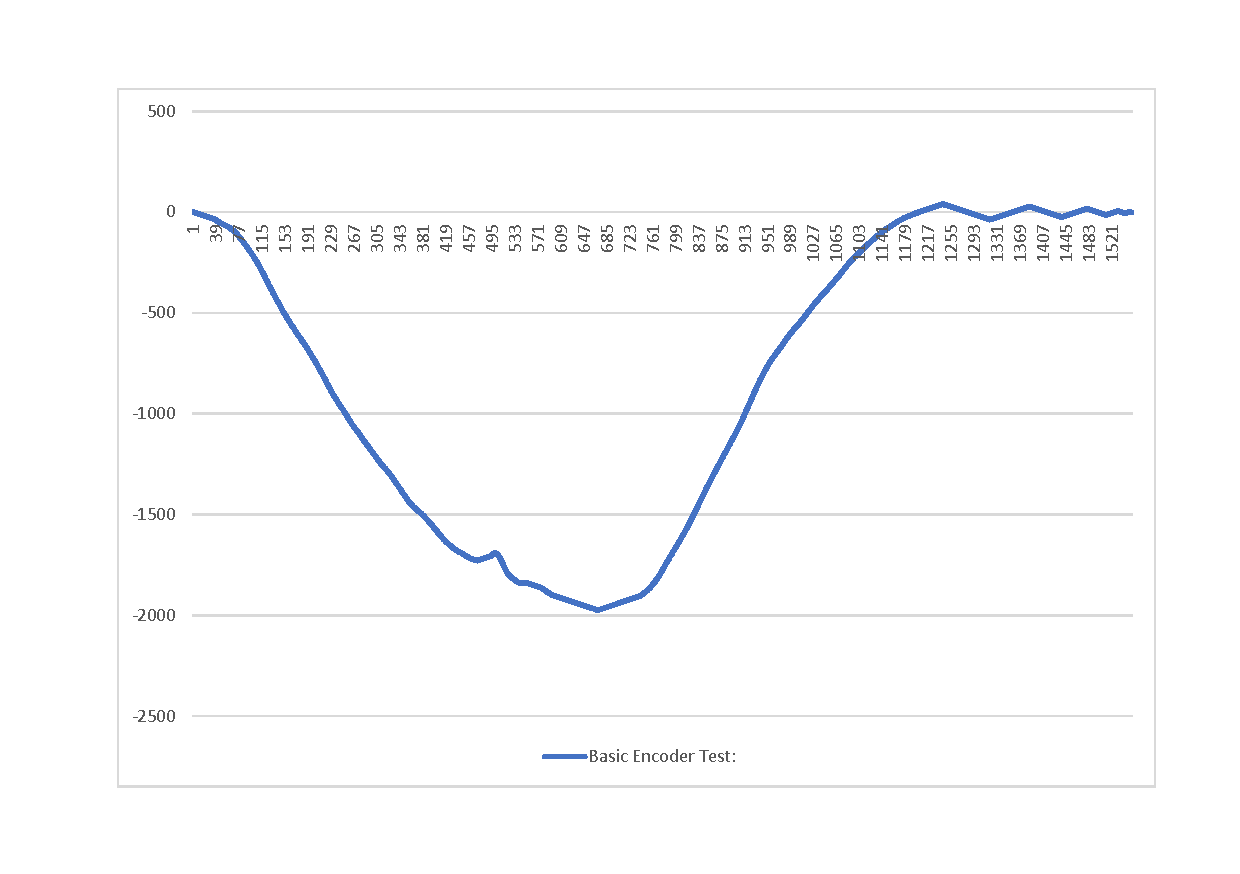
\includegraphics[width=14cm, height=10cm]{pruebasensor}
	\caption{Diagrama de adquisi'on de datos del sensor HEDM-5500}
	\label{fig:adqsens}
\end{figure}
\end{center}
\subsection{An'alisis de los datos obtenidos de los sensores}
Se puede observar una correlaci'on entre los datos obtenidos en la interfaz serial de Arduino IDE (Fig. \ref{fig:dard}) con los puntos de resoluci'on del sensor mostrados en HMI Fig. \ref{fig:dHMI}; cabe resaltar que estos datos fueron enviados a trav'es de CAN hacia el nodo central y luego a la HMI.
\begin{figure}[ht]
	\centering
		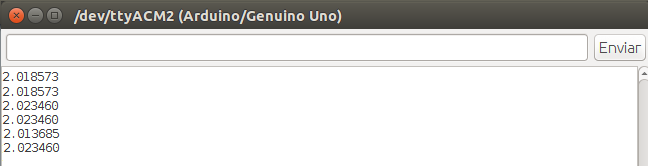
\includegraphics[scale=0.9]{datoshmi}
	\caption{Datos obtenidos por Arduino IDE}
	\label{fig:dard}
\end{figure}
\begin{figure}[ht]
	\centering
		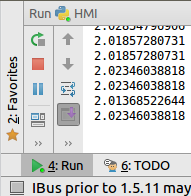
\includegraphics[scale=1]{datoshmi2}
	\caption{Datos obtenidos por HMI}
	\label{fig:dHMI}
\end{figure}

\section{Prueba del sistema simulado de control}

\subsection{Prueba del controlador en estado estable para el sistema desarrollado en Matlab}
\setlength{\parskip}{0.4cm}
En el cap'itulo anterior se mostr'o la utilidad de Matlab a la hora de obtener ganancias de un sistema en espacio de estados, tambi'en se puede a'nadir el siguiente c'odigo para obtener la simulaci'on en condiciones iniciales dadas y el tracking a una se'nal de entrada:

 {\tiny
\lstset{language=Matlab, breaklines=true, basicstyle=\footnotesize}
\begin{lstlisting}[frame=single]
%% 2. SIMULATION IN FRONT OF GIVEN CONDITIONS
x = [1; 1]; %given initial conditions
history = []; %buffer initialization
history = [history sys_d.c*x];

for i = 0 : tick : tTop
    u = -K*x; %applies control
    x = sys_d.a*x+sys_d.b*u;
    y = sys_d.c*x;
    history = [history y]; %updates buffer
end

time = 0:tick:tTop+tick;
figure
plot(time, history(1,:));
xlabel('Time [s]');
ylabel('x[1]');
legend('State');
axis([0 tTop -1 1])

%% 3. SIMULATION TRACKING A REFERENCE SIGNAL
tTop = 5;
x = [0; 0]; %given initial conditions

history = []; %buffer initialization
history = [history x];

ref = 0;
real_ref = ref - 0.5;
refHist = [];
refHist = [refHist, ref];

u = 0;
controlHist = [];
controlHist = [controlHist, u];

for i = 0 : tick : tTop
    if mod(i,1) == 0 && i ~= 0
        ref = ~ref;
        real_ref = ref - 0.5; %to simulate the behavior in the flexboards
    end
    u = K(1)*(real_ref-x(1)) - K(2)*x(2);
    x = sys_d.a*x+sys_d.b*u;
    history = [history x]; %updates buffer
    refHist = [refHist real_ref];
    controlHist = [controlHist u];
end

time = 0:tick:tTop+tick;

figure
hold on
plot(time, history(1,:));
plot(time, refHist(1,:),'color', 'red')
plot(time, controlHist(1,:),'color', 'green')
xlabel('Time [s]');
ylabel('Voltage');
legend('State','Reference','Control');
axis([0 tTop -2 2])
\end{lstlisting}
}
\subsection{Resultados adquiridos de Matlab}
A continuaci'on se muestran los datos obtenidos de Matlab
 {\tiny
\lstset{language=Matlab, breaklines=true, basicstyle=\footnotesize}
\begin{lstlisting}[frame=single]
Crank system is controllable!
Convergence was reached at
iter =  2194
Crank control gains:
K_ = [ 72.49, 25.91, 14.25, -2.096] 
KI_ = 0.9615
eigenvalues =    0.9669 + 0.0000i
   0.9817 + 0.0277i
   0.9817 - 0.0277i
   0.9920 + 0.0303i
   0.9920 - 0.0303i
\end{lstlisting}
}

\subsection{Gr'afico obtenido de la simulaci'on}
Dando como resultado que el sistema sea completamente controlable como muestra la Fig. \ref{fig:simu}:

\begin{center}
\begin{figure}[ht]
	\centering
		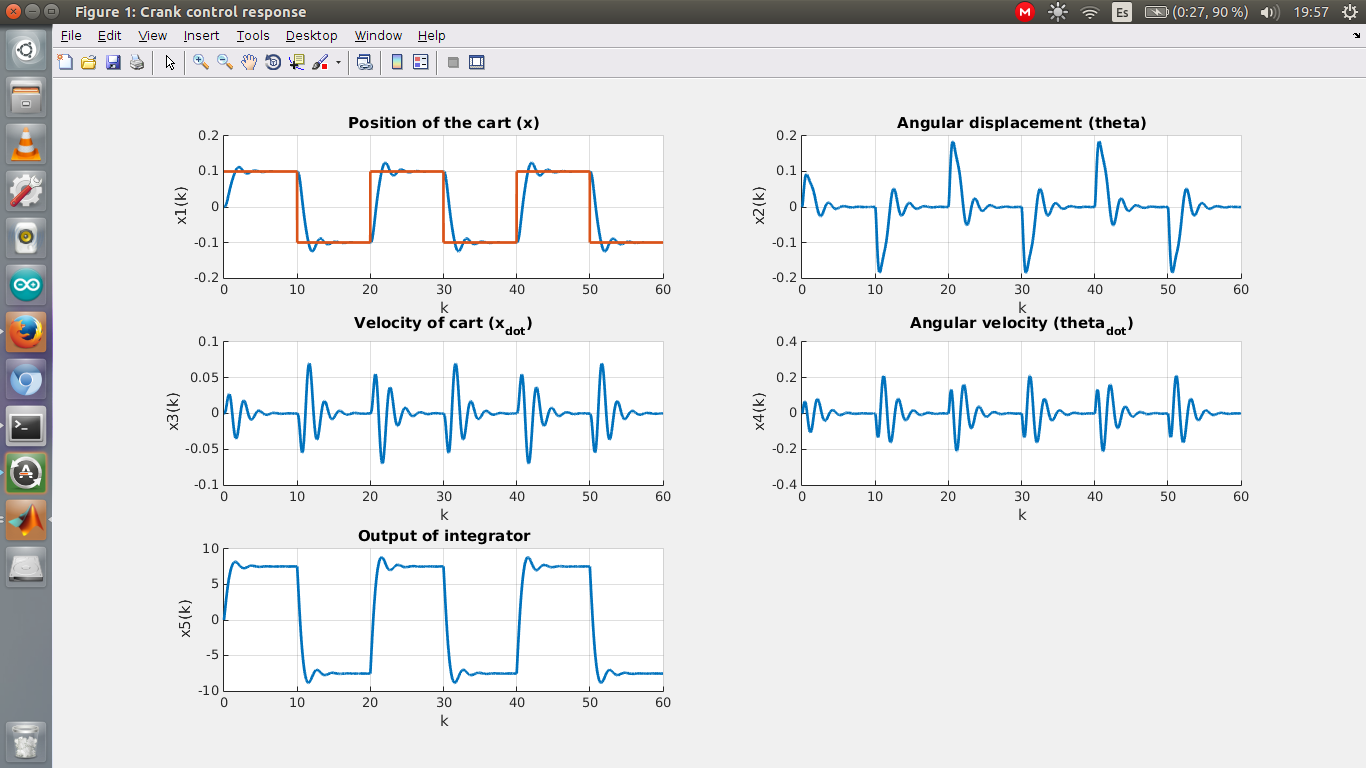
\includegraphics[width=15cm, height=10cm]{simu}
	\caption{Simulaci'on obtenida con Matlab}
	\label{fig:simu}
\end{figure}
\end{center}
\subsection{An'alisis de los resultados}
Los resultados obtenidos por Matlab muestran que el sistema es controlable, con una itinerancia de software de 2149; donde se encontraron los polos del sistema as'i como sus ganancias, las cu'ales fueron puestas en un sistema de realimentaci'on cerrado y simulado por Matlab Fig. \ref{fig:simu}.


\section{Prueba del sistema real con las ganancias obtenidas}
Prueba del sistema real con las ganancias obtenidas en el cap'itulo anterior en donde fueron modificadas para reducir el tiempo de estabilizaci'on en estado estable, dando la siguiente tabla \ref{tabla:pruebag}:

\begin{table}[htbp]
\begin{center}
\begin{tabular}{c c c c c c c}
\hline
Prueba &G1CarPos & G2CarVel& G3RosPos & G4RosVel & G5error& Tiempo Estabilizacion(seg)\\
\hline 
1 &59.86&17.9&10.17&-3.713&0.98& Inestable\\
2 &59.86&17.9&-10.17&-3.713&0.15& 20 \\
3 &59.86&17.9&-40.17&-3.713&0.15& 14 \\
4 &59.86&17.9&-40.17&-10.713&0.15& 13\\
5 &59.86&17.9&-40.17&-1.713&0.15& 15\\
6 &59.86&17.9&-40.17&-5.713&0.15& 15\\
7 &59.86&17.9&-40.17&-7.713&0.15& 14\\
8 &59.86&17.9&-40.17&-20.713&0.15& 11\\
9 &59.86&17.9&-40.17&-10.713&0.1& 14\\
10 &59.86&17.9&-40.17&-3.713&0.08& 12\\
11 &59.86&17.9&-3.17&-3.713&0.1& 20\\
12 &59.86&17.9&-40.17&-3.713&0.25& Inestable\\
\hline 
\end{tabular}
\caption{Tabla comparativa de ganancias}
\label{tabla:pruebag}
\end{center}
\end{table}

\subsection{An'alisis de los ganancias modificadas en el sistema real}
 Los datos de la tabla \ref{tabla:pruebag} muestra que las ganancias m'as cr'iticas son G3RosPos y G5error; tomando la primera valores menores a 0 el sistema se vuelve inestable y para la segunda con valores mayores a 1.5 sucede lo mismo. El mejor tiempo de estabilizaci'on se obtuvo con  G3RosPos=-40.17,G2CarVel=-20.713 y G5error =0.15 con un tiempo de estabilizaci'on de 11 seg. 


\section{An'alisis costos}
A continuaci'on se detallan los costos del trabajo realizado en la tabla \ref{tabla:costos}:

\begin{table}[htbp]
\begin{center}
\begin{tabular}{c c c c c c c c}
\hline
Egresos &Mes1&Mes2&Mes3&Mes4&Mes5&Mes6&Total\\
 &USD&USD&USD&USD&USD&USD&USD\\
\hline 
Materia prima & 200 & & & &200 && 400 \\
Mano de obra directa &  & & & & 20&& 20 \\
Mano de obra indirecta &  & & & & &&0\\
Materiales de oficina & 10 &10 &10 &5 &20 &5&60\\
\hline 
 &&&&&&Costo&480\\
&&&&&&Precio&520\\
\hline 
\end{tabular}
\caption{Tabla de costos}
\label{tabla:costos}
\end{center}
\end{table}